\documentclass[assd_tp2_main.tex]{subfiles}

\begin{document}

\section{Síntesis basada en muestras}


La síntesis basada en muestras permite que a partir de una muestra con cierta duración, se pueda obtener una nota distinta a la original y con distinta duración achicando o alargando la muestra. Para ello es necesario poder modificar tanto la frecuencia fundamental como la duración independientemente.

La duración de la nota se puede cambiar a partir del resampleo. Al resamplear una señal, no solo se modifica la duración, sino que también la frecuencia fundamental de la misma.

\begin{figure}[H]	
	\centering
	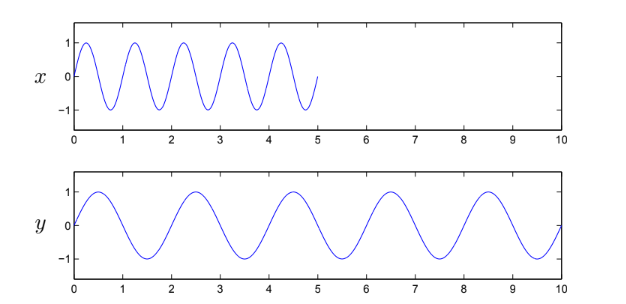
\includegraphics[scale=1]{graficos/EJ6/timestretch.png}
	\caption{x está sampleada a una frecuencia de 22050 Hz y tiene una frecuencia de 1Hz. Resampleando la señal con una frecuencia de 44100 Hz se obtiene la señal y que tiene el doble de duración que x y la mitad de frecuencia (0.5Hz)}
\end{figure}

Por lo tanto, una vez cambiada la frecuencia mediante dicha técnica, se necesita un algoritmo que sea capaz de cambiar la duración del audio sin modificar nuevamente su frecuencia. 

\subsection{Escalamiento Temporal (TSM)}

Existe una gran variedad de algoritmos que cumplen con la tarea de modificar la duración de un audio. Ya se mencionó el ejemplo del resampleo, a continuación se analizará otro algoritmo denominado Overlap-Add (OLA) que elimina en la mayor escala posible el problema de la alteración en la frecuencia.

\subsubsection{Overlap-Add (OLA)}

La idea de este algoritmo consiste en cortar la señal de entrada en pequeños segmentos y luego encadenarlos para obtener la longitud deseada.

\begin{figure}[H]	
	\centering
	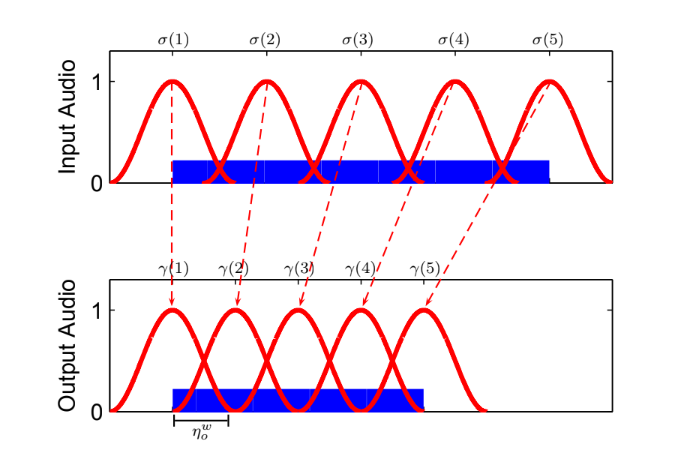
\includegraphics[scale=0.75]{graficos/EJ6/OLA.png}
	\caption{Algoritmo OLA}
\end{figure}

Los parámetros que utiliza el algorimo son la muestra original, un factor de solapamiento, una función ventana y una función que 'mapea' los tiempos de la escala original a la nueva escala. Matemáticamente se puede escribir esta síntesis como:

\begin{equation}
y(n)=\frac{\sum_{k=1}^{len(\sigma)} \omega(n - \gamma (k)) x(n-\gamma (k) + \sigma (k))}{\sum_{k=1}^{len(\sigma)}\omega(n - \gamma (k))}
\end{equation}

Donde $x$ es la señal de muestra, $\omega$ es la función ventana  (en este caso utilizamos la ventana Hann, cuya longitud debe ser mayor que a lo sumo un periódo de la señal),  $\sigma$ es el vector que contiene las posiciones de las ventanas en la escala de entrada y $\gamma$ es el vector con las posiciones de las ventanas en la escala de salida. Estos dos están vinculados mediante:
\begin{equation}
\sigma(n)= \tau^{-1}\left(\gamma(n)\right)
\end{equation}
Donde $\tau$ es la función que convierte los puntos de la escala original a la deseada.

Entonces, como muestra la ecuación, se toma segmentos del original definidos por el tamaño y la amplitud de la ventana utilizada y luego se solapan estos segmentos de acuerdo lo indica la función $\tau$, que es la que estira o acorta la escala de acuerdo con la duración que se desea para la salida.

La calidad del sonido que se obtiene a partir de este algoritmo es más aceptable para muestras que no tienen naturaleza armónica como es por ejemplo una señal de voz. Pero cuando se trata de estiramiento temporal para una señalcon contenido armónico, como por ejemplo una nota musical, se introducen en la salida ciertos defectos como modulación y saltos de fase producidos por el solapamiento de las ventanas.

A continuación se muestran los resultados obtenidos para una señal con contenido armónico, donde se utilizó como señal de entrada una senoidal pura, y para una señal no armónica, utilizando como muestra una nota de voz.

\begin{figure}[H]
\centering
  \begin{minipage}{0.4\textwidth}
    \centering
    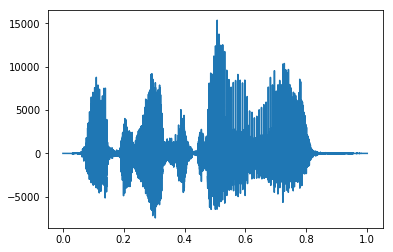
\includegraphics[width=1\textwidth]{graficos/EJ6/in.png}
    \caption{Señal de voz entrada}
    \label{fig:uno}
  \end{minipage}%
  \hspace{5mm}
  \begin{minipage}{0.4\textwidth}
    \centering
    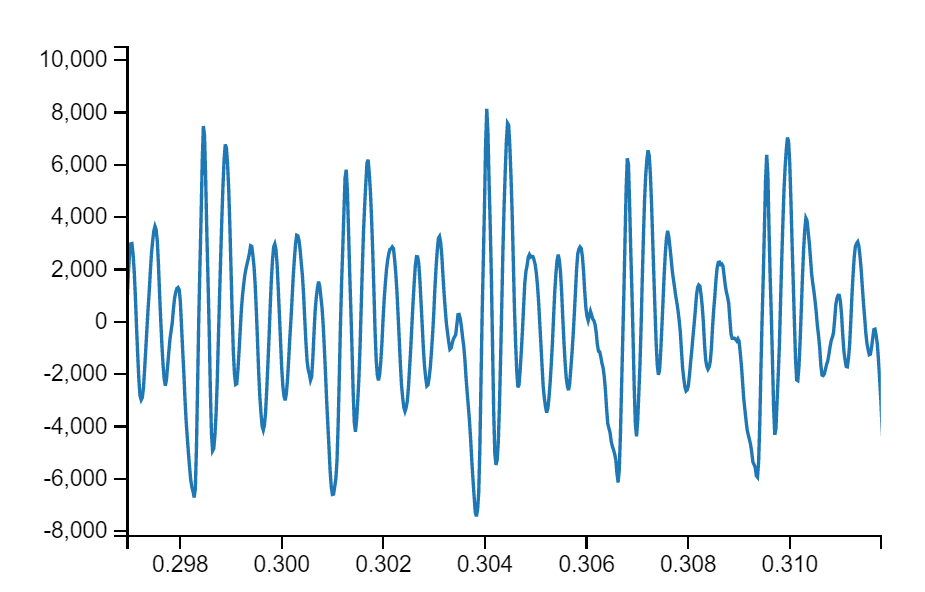
\includegraphics[width=1\textwidth]{graficos/EJ6/inzoom.png}
    \caption{Señal de entrada con zoom}
    \label{fig:dos}
  \end{minipage}
\end{figure}

\begin{figure}[H]
\centering
  \begin{minipage}{0.4\textwidth}
    \centering
    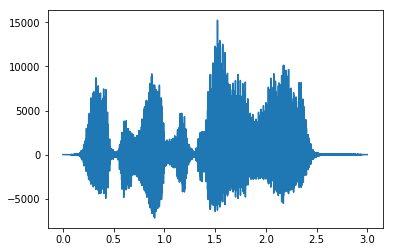
\includegraphics[width=1\textwidth]{graficos/EJ6/outx3.png}
    \caption{Señal a la salida con el triple de duración que la entrada}
    \label{fig:uno}
  \end{minipage}%
  \hspace{5mm}
  \begin{minipage}{0.4\textwidth}
    \centering
    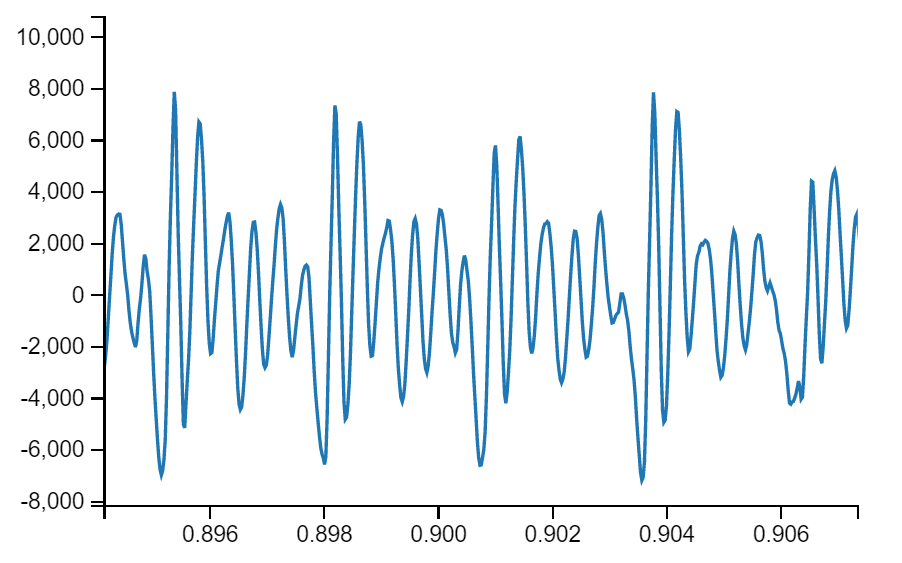
\includegraphics[width=1\textwidth]{graficos/EJ6/outx3zoom.png}
    \caption{Señal de salida con zoom}
    \label{fig:dos}
  \end{minipage}
\end{figure}

\begin{figure}[H]
\centering
  \begin{minipage}{0.4\textwidth}
    \centering
    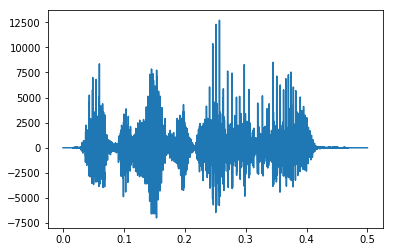
\includegraphics[width=1\textwidth]{graficos/EJ6/outmitad.png}
    \caption{Señal a la salida con la mitad de duración que la entrada}
    \label{fig:uno}
  \end{minipage}%
  \hspace{5mm}
  \begin{minipage}{0.4\textwidth}
    \centering
    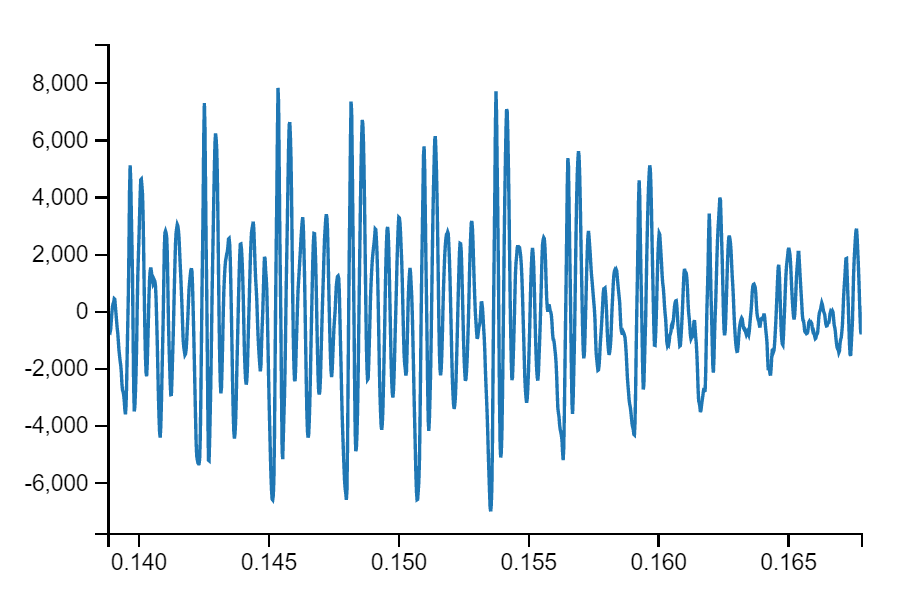
\includegraphics[width=1\textwidth]{graficos/EJ6/outmitadzoom.png}
    \caption{Señal de salida con zoom}
    \label{fig:dos}
  \end{minipage}
\end{figure}

\begin{figure}[H]	
	\centering
	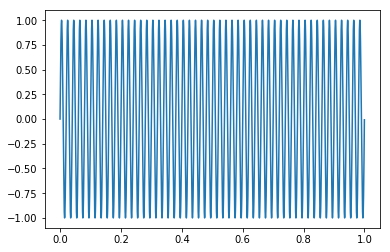
\includegraphics[scale=0.5]{graficos/EJ6/senoin.png}
	\caption{Señal senoidal de entrada (50Hz)}
\end{figure}

\begin{figure}[H]
\centering
  \begin{minipage}{0.4\textwidth}
    \centering
    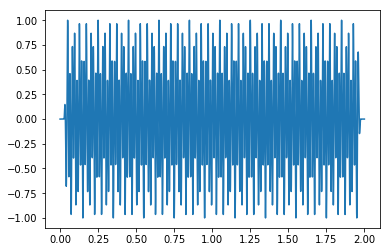
\includegraphics[width=1\textwidth]{graficos/EJ6/senodoble.png}
    \caption{Señal a la salida con el doble de duración que la entrada}
    \label{fig:uno}
  \end{minipage}%
  \hspace{5mm}
  \begin{minipage}{0.4\textwidth}
    \centering
    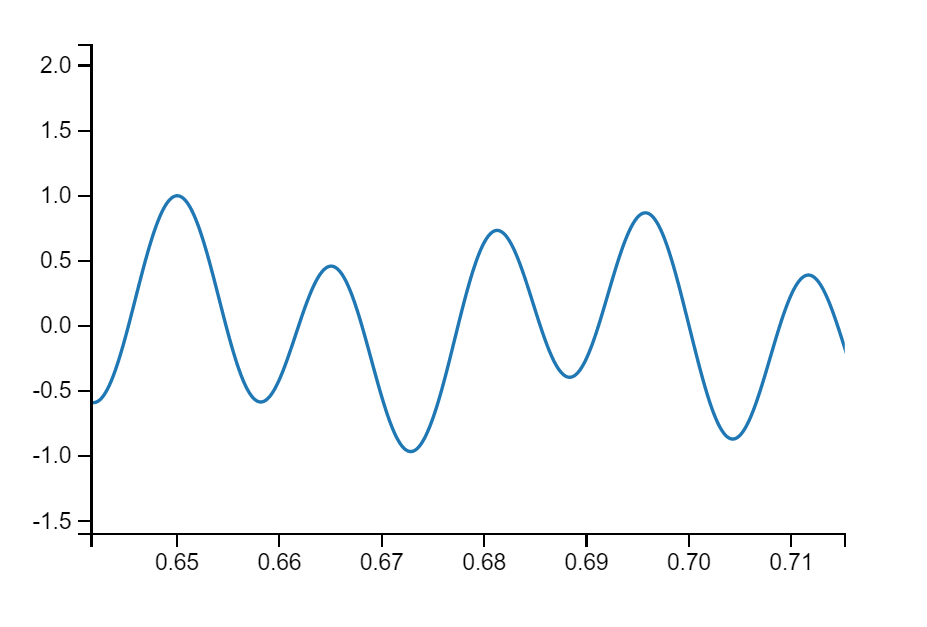
\includegraphics[width=1\textwidth]{graficos/EJ6/senodoblezoom.png}
    \caption{Señal de salida con zoom}
    \label{fig:dos}
  \end{minipage}
\end{figure}

\begin{figure}[H]	
	\centering
	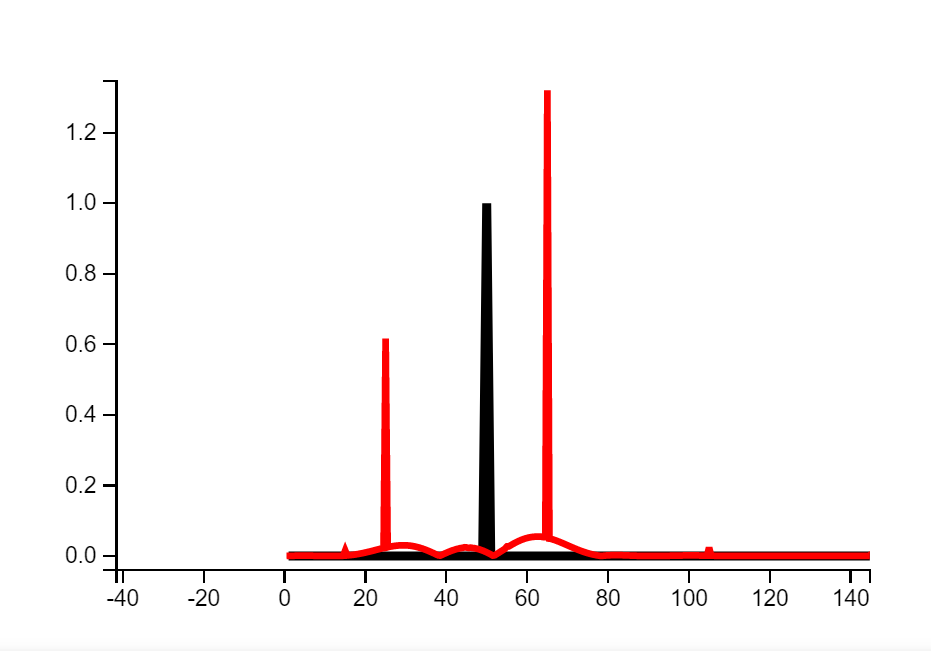
\includegraphics[scale=0.5]{graficos/EJ6/senoespectro.png}
	\caption{Espectro de las señales de entrada y salida. La negra es la entrada y la roja es la salida}
\end{figure}

Como se mencionó anteriormente, el algoritmo es mas fiel a la forma de la señal cuando esta no es de naturaleza armónica, pero introduce distorsiones cuando si lo es. En las fotos se puede observar la modulación presente en la salida.

Existen otros algorimos más complejos que tienen como objetivo evitar este mal comportamiento de OLA en las señales con contenido armónico, uno de ellos es WSOLA.

Su funcionamiento es muy similar al de OLA, pero para que los segmentos sean lo más parecidos posible en la zona que se solapan y el resultado sea más satisfactorio, permite que los estos se puedan desplazar una cierta tolerancia temporal respecto de la posición original. Para encontrar este desplazamiento se busca la correlación máxima entre dos fragmentos adyacentes.

Matemáticamente se describe:
\begin{equation}
y(n)=\frac{\sum_{k=1}^{len(\sigma)} \omega(n - \gamma (k)) x(n-\gamma (k) + \sigma (k) + \Delta_{k})}{\sum_{k=1}^{len(\sigma)}\omega(n - \gamma (k))}
\end{equation}

Es muy similar al OLA, salvo por los desplazamientos $\Delta_{k}$.

\subsection*{Referencias}
Time-scale Modification Algorithms for music audio signals by Jonathan Driedger



\end{document}

